\section{Introduction}
\label{sec:introduction}

% state the learning objective 
The objective of this laboratory assignment is to study a circuit containing a voltage source $V_A$, a current-controlled voltage source $V_C$, a current source $I_D$ and a voltage-controlled current source $I_B$ connected to different fixed value resistors $R_1$, $R_2$, $R_3$, $R_4$, $R_5$, $R_6$, $R_7$. The circuit can be seen in Figure~\ref{fig:rc}.

**************************************************************************
In Section~\ref{sec:analysis}, a theoretical analysis of the circuit is
presented. In Section~\ref{sec:simulation}, the circuit is analysed by
simulation, and the results are compared to the theoretical results obtained in
Section~\ref{sec:analysis}. The conclusions of this study are outlined in
Section~\ref{sec:conclusion}.

\begin{figure}[h] \centering
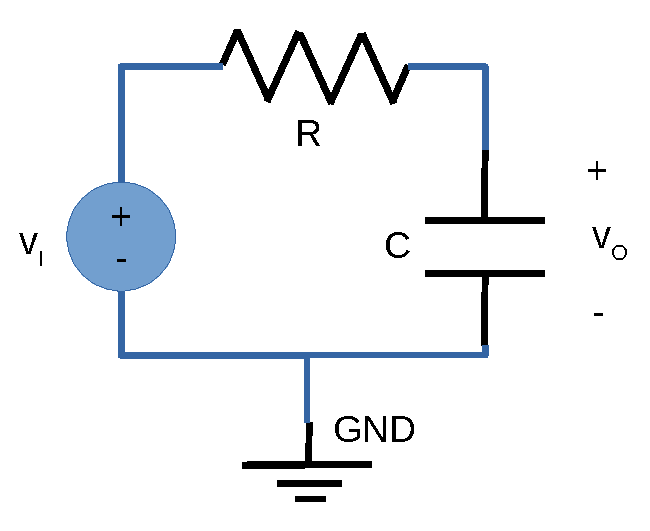
\includegraphics[width=0.4\linewidth]{rc.pdf}
\caption{Voltage driven serial RC circuit.}
\label{fig:rc}
\end{figure}
**************************************************************************

The Mesh Current Method is another well-organized method for solving a circuit and is based on Kirchhoff's Voltage Law (KVL). To apply this method, we need to define what mesh current is. When we use the term mesh current, we are referring to an imagined current flowing around a loop. To aplly this first step of this method, we first need to identify and distinguish a loop from a mesh. A loop correspond to any closed path around the circuit and, to trace it, we start at any component terminal and trace a path through connected elements until we get back to the starting point. A loop is allowed to go through an element just one time. That leads us to the definition of a restricted kind of loop, a mesh, which contains no other loops.

The implementation of the Mesh Current Method to analyse the circuit was done following the common sequence of steps, summarized below.
    Identify the meshes.
    Assign a current variable to each mesh, using a consistent direction (clockwise or counterclockwise).
    Write Kirchhoff's Voltage Law equations around each mesh .
    Solve the resulting system of equations for all mesh currents.
    Solve for any element currents and voltages you want using Ohm's Law.

The Node Voltage Method is another way to analyze a circuit. This method is based on Kirchhoff's Current Law (KCL). To apply this method, we need to define what node voltage is. When we use the term node voltage, we are referring to the potential difference between two nodes of a circuit. We select one of the nodes in our circuit to be the reference node and, therefore, all the other node voltages are measured with respect to the referenced one. This reference node is called the ground node and, as it gets the ground symbol in Figure~\ref{fig:rc}, corresponds to the node between resistor $R_1$ and voltage source $V_A$. The potential of the ground node is defined to be null and the potentials of all the other nodes are measured relative to ground.

The implementation of the Node Voltage Method to analyse the circuit was done following the common sequence of steps, summarized below.
    Assign a reference node (ground).
    Assign node voltage names to the remaining nodes.
    Solve the easy nodes first, the ones with a voltage source connected to the reference node.
    Write Kirchhoff's Current Law for each node. Do Ohm's Law in your head.
    Solve the resulting system of equations for all node voltages.
    Solve for any currents you want to know using Ohm's Law.



